\documentclass[class=article , crop=false, titlepage, twoside, multi={itemize, figure, verbatim}, float=false]{standalone}
    %
\usepackage{import} % Required for importing other .tex docs.  (import uses everything bw Begin and End Doc)
\usepackage{float} % Required for specifying the exact location of a figure or table
\usepackage{graphicx} % Required for including images
\usepackage{wrapfig}
\usepackage[pdftex,breaklinks,colorlinks=true,linkcolor=black,citecolor=blue,urlcolor=red,linktocpage=false,pagebackref=true,filecolor=magenta]{hyperref}%http://www.tug.org/applications/hyperref/manual.html#x1-100003.6
\usepackage{cite}
\usepackage[toc,title,page]{appendix}
\usepackage{pdfpages} % enables loading a pdf into the doc
\usepackage{makeidx}
\usepackage{glossaries} % must be after hyperref
\usepackage{blindtext}
\usepackage{enumitem}
%\usepackage{caption}

%\setlist[description]{leftmargin=\parindent,labelindent=\parindent}

%\renewcommand*{\bibname}{References} % renames the bibliography

\newcommand{\HRule}{\rule{\linewidth}{0.5mm}} % Command to make the lines in the title page

\graphicspath{{img/}{GIS_ChampionSection/img/}{awardsChapter/GIS_ChampionSection/img/}{brandPart/awardsChapter/GIS_ChampionSection/img/}{img/}{pairedProgSection/img/}{methodChapter/pairedProgSection/img/}{methodPart/methodChapter/pairedProgSection/img/}{documentationSection/img/}{methodChapter/documentationSection/img/}{methodPart/methodChapter/documentationSection/img/}{docStorageOrgSection/img/}{methodChapter/docStorageOrgSection/img/}{methodPart/methodChapter/docStorageOrgSection/img/}{QGisSection/img/}{toolsChapter/QGisSection/img/}{servicePart/toolsChapter/QGisSection/img/}{ESRISection/img/}{toolChapter/ESRISection/img/}{servicePart/toolChapter/ESRISection/img/}{../../../../source/}{../../source/}{servicePart/applicationsChapter/treasurerSection/img/}}

%\setlength\parindent{0pt} % eliminates indents

    %
\def\titlename{GDB Maintenance\\ \medskip\large Enterprise Geodatabase Maintenance}
    %
\title{\HRule % Horizontal Line added
\\[.4cm] % space
\begin{figure}[H] % included image
\begin{center}	% centered horizontally
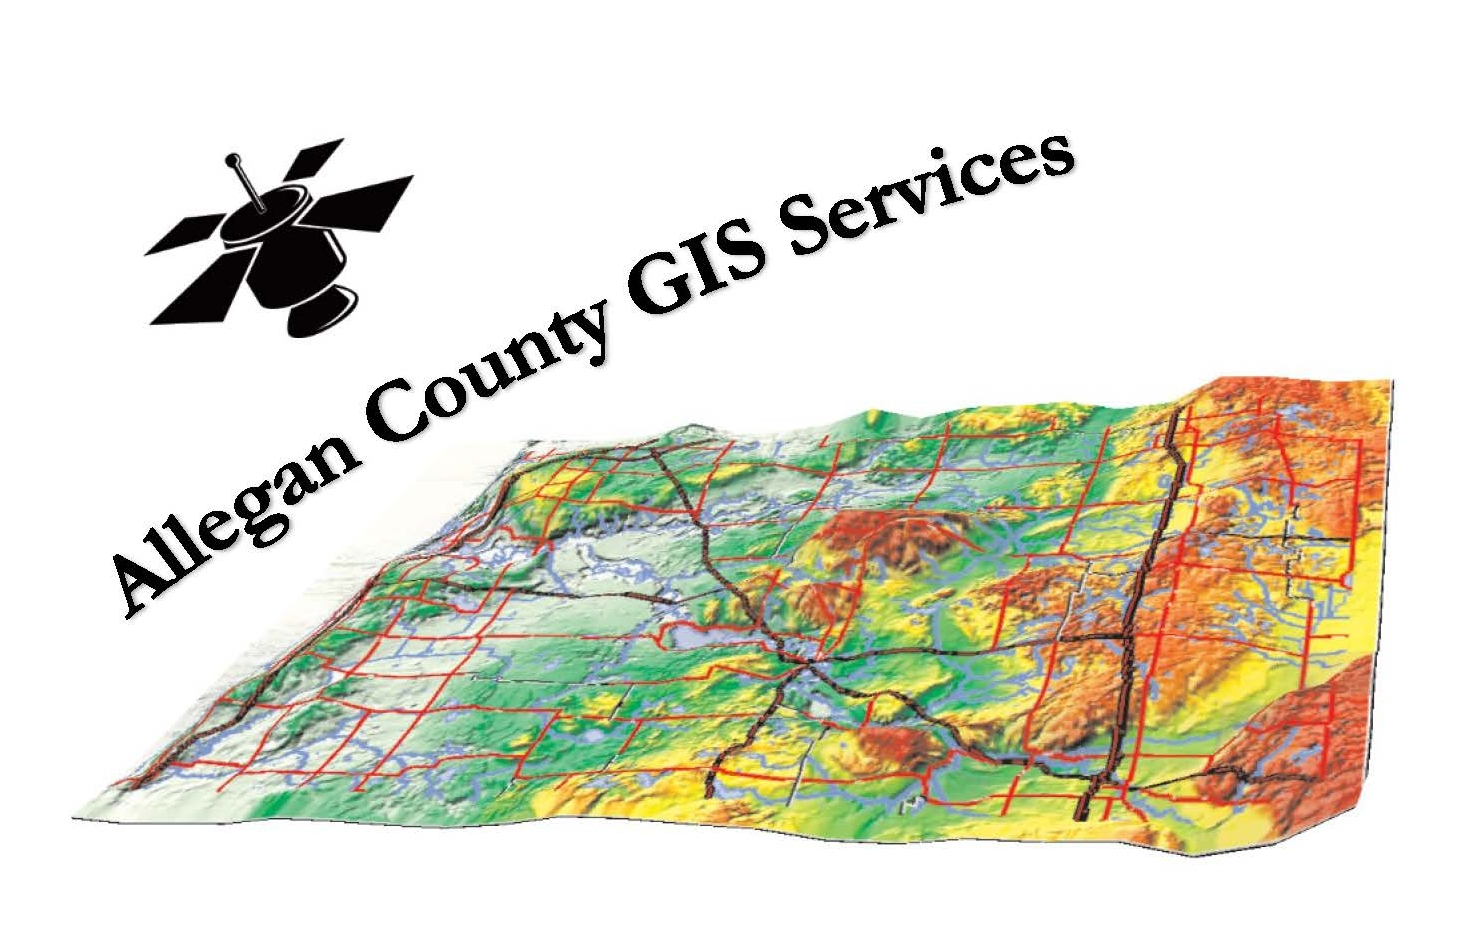
\includegraphics[scale=.45]{GIS_Logo_better.jpg}
\end{center}
\end{figure}
\Huge \bfseries \titlename \\ % Title text
\HRule \\[.4cm] % Horizontal Line added
\author{\Large Allegan County GIS \\\Large www.allegancounty.org/gis} % defines author
}  % inputs common title
\setcounter{tocdepth}{5}  % subparagraph and down
\begin{document}% document begins
    %
\ifstandalone
\frontmatter % turns off chapter numbering and uses roman numerals for page numbers
\maketitle % creates title page and blank page after title page
\tableofcontents % creates TOC and blank page
\clearpage
\mainmatter % turns on chapter numbering, resets page numbering and uses arabic numerals for page numbers
\fi
    %
\subsection{Enterprise Geodatabase Maintenance}
    %
\subsubsection{Enterprise Geodatabase Compression Routine}
    %
\paragraph[Disconnect Users]{Disconnect All Users\texorpdfstring{\\}{}}
    %
\noindent {\Large To disconnect the GIS Server, stop all services}
    %
\begin{itemize}
    %
\item In ArcGIS Server Manager $\Rightarrow$  Site $\Rightarrow$ GIS Server $\Rightarrow$ Machines $\Rightarrow$ Stop all Services
    %
\end{itemize}
    %
\begin{figure}[h!]
\centering
    \includegraphics[width=1\textwidth]{stopArcGisServer.png}
    %
\vspace*{-10mm}\caption{Stop ArcGIS Server}

\end{figure}
%\clearpage
\paragraph*{}Use the Search tool to find the Rebuild Indexes Tool
\begin{figure}[h!]
\centering
    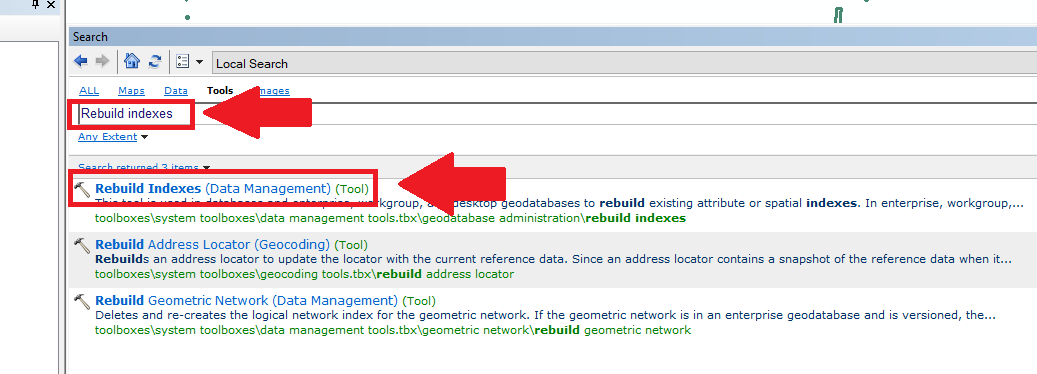
\includegraphics[width=1\textwidth]{findRebuildIndexesTool.png}
    %
\vspace*{-10mm}\caption{Find Rebuild Indexes Tool}

\end{figure}
\clearpage
    %
    %
\paragraph[Rebuild Indexes]{Rebuild Indexes\texorpdfstring{\\}{}}
    %
\noindent Select Connection $\Rightarrow$  Include System Tables $\Rightarrow$ Select All $\Rightarrow$ Press OK
    %
\begin{figure}[h!]
\centering
	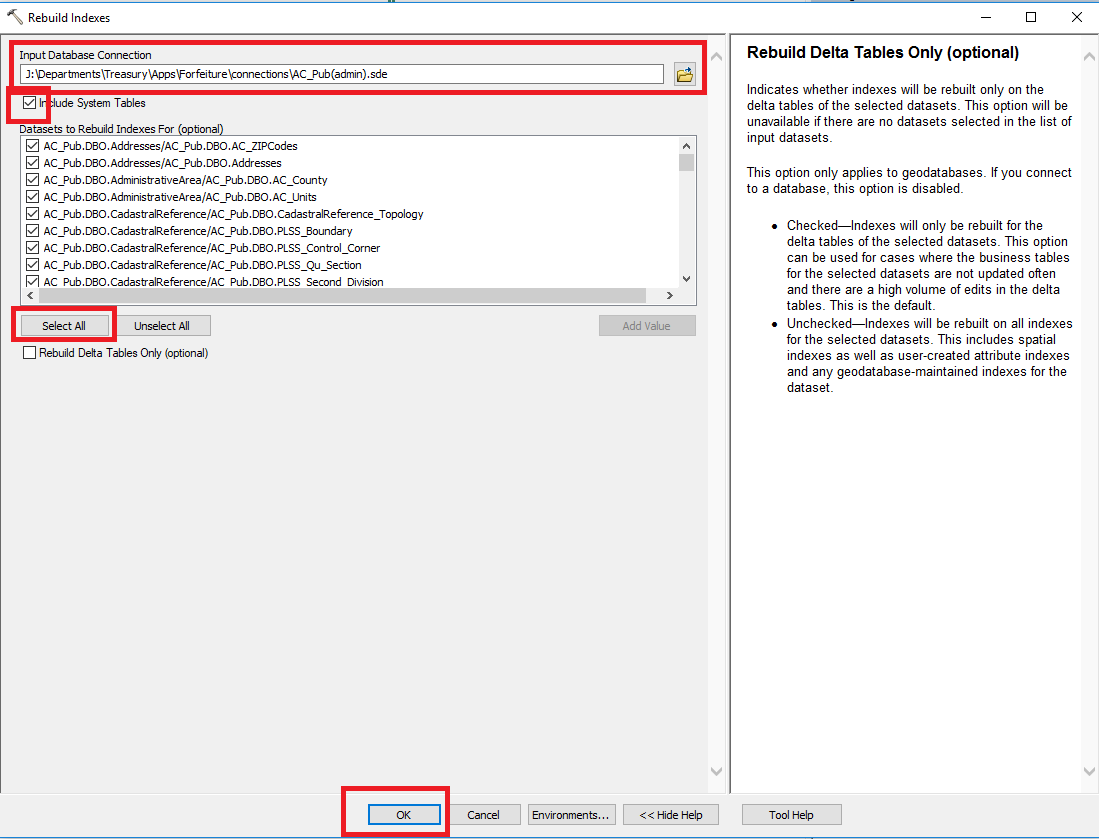
\includegraphics[width=.9\textwidth]{rebuildIndexesToolOperation.PNG}
\caption{Rebuild Indexes Tool Operation}
\end{figure}
    %
\clearpage
    %
\paragraph[Recalculate Statistics]{Recalculate Statistics\texorpdfstring{\\}{}}
\noindent In the Analyze Datasets Tool:\\
\noindent Select Connection $\Rightarrow$  Include System Tables $\Rightarrow$ Select All $\Rightarrow$ Press OK
\begin{figure}[h!]
\centering
	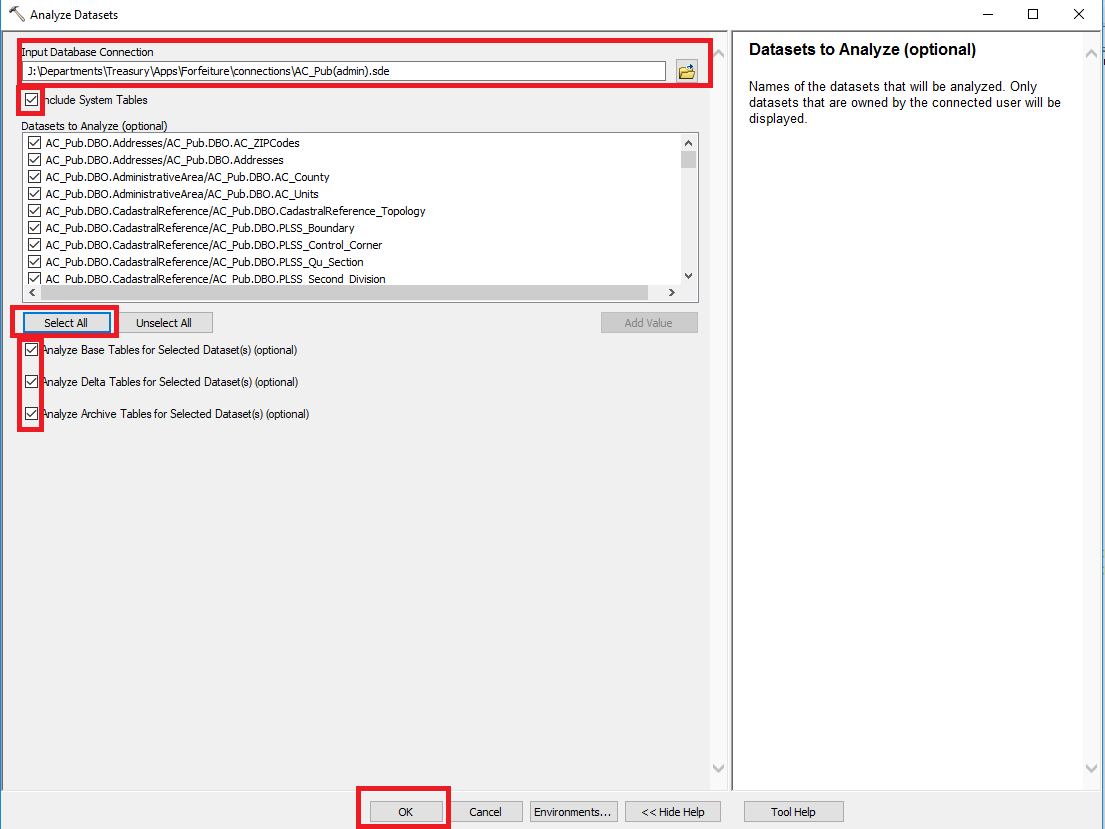
\includegraphics[width=.9\textwidth]{recalculateStatistics.PNG}
\caption{Recalculate Statistics}
\end{figure}
\clearpage
    %
    %
\paragraph[Compress]{Compress\texorpdfstring{\\}{}}
    %
\noindent  Select Connection $\Rightarrow$  Press OK
\begin{figure}[h!]
\centering
	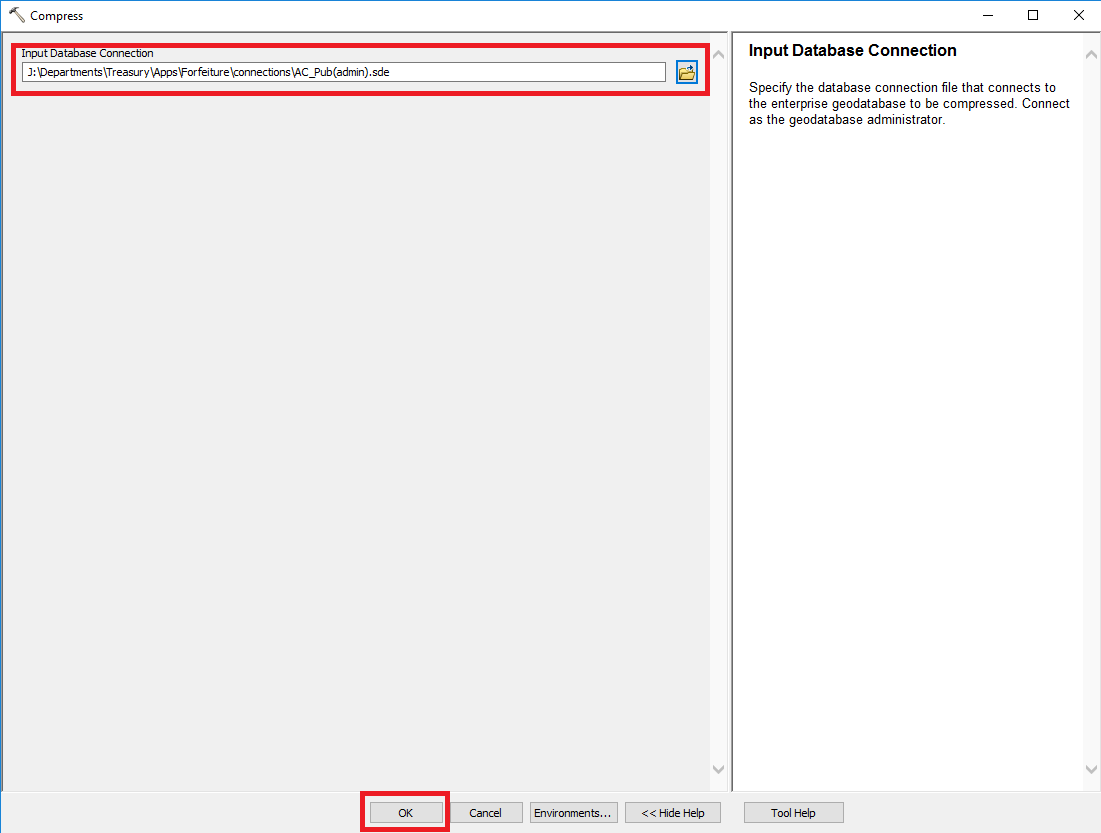
\includegraphics[width=.75\textwidth]{compress.PNG}
\caption{Compress}
\end{figure}
    %
\clearpage
    %
    %
\paragraph{Rebuild Indexes Again}
\begin{figure}[h!]
\centering
	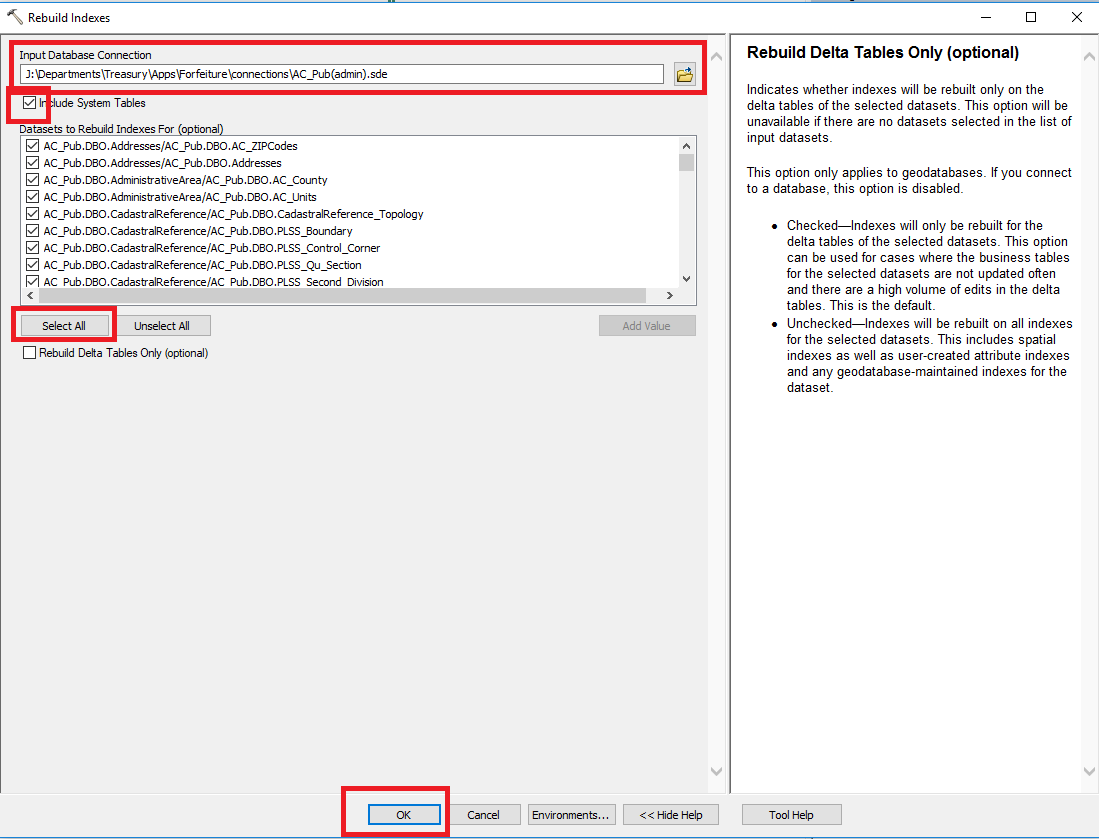
\includegraphics[width=.75\textwidth]{rebuildIndexesToolOperation.PNG}
\caption{Rebuild Indexes Tool Operation}
\end{figure}
\clearpage
    %
    %
\paragraph[Recalculate Statistics]{Recalculate Statistics Again\texorpdfstring{\\}{}}
    %
\noindent In the Analyze Datasets Tool:\\
    %
\noindent Select Connection $\Rightarrow$  Include System Tables $\Rightarrow$ Select All $\Rightarrow$ Press OK
    %
\begin{figure}[h!]
\centering
	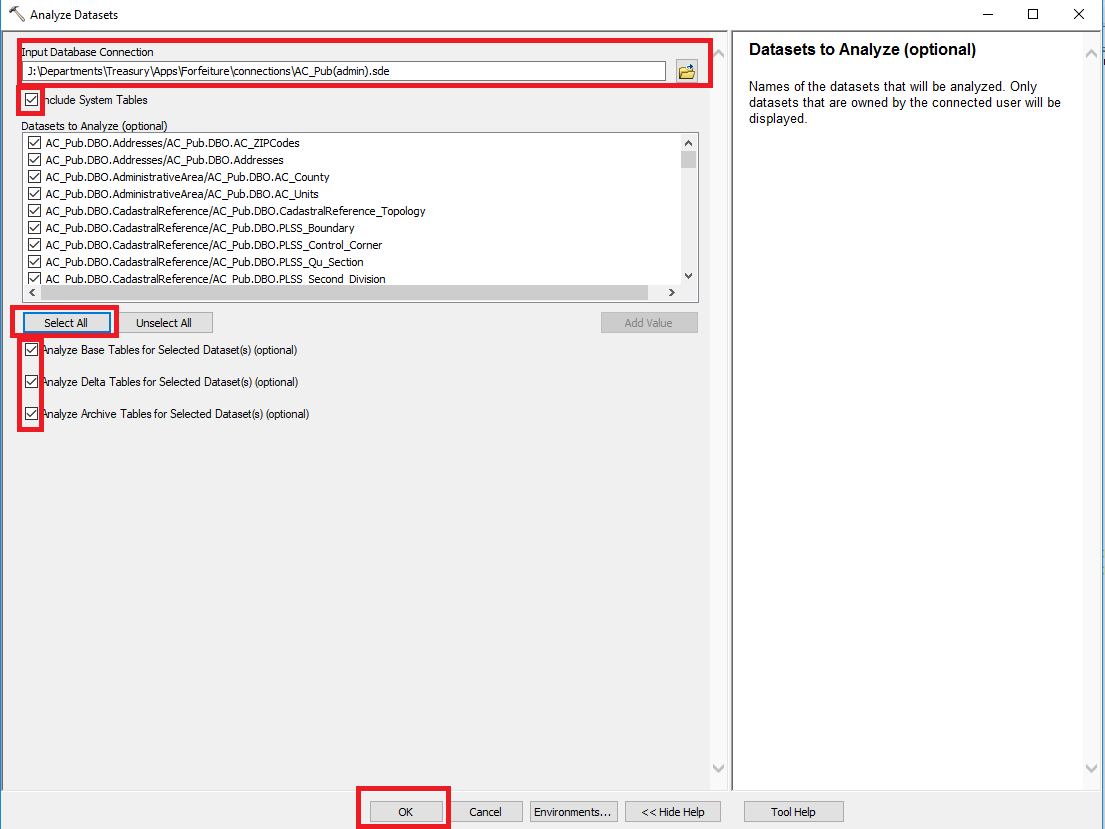
\includegraphics[width=.95\textwidth]{recalculateStatistics.PNG}
\caption{Recalculate Statistics}
\end{figure}
    %
\clearpage
    %
    %
\end{document}
